\chapter{Rilascio}
\label{chap:rilascio}
In questa sezione verrà presentato il rilascio del prodotto finale, concludendo infine con un esempio di integrazione dell'SDK
all'interno di un prodotto \textit{Datasoil S.rl.} operativo.

\section{Rilascio SDK}
Al fine di rilasciare un \textit{package}, è necessario effettuare la \textit{build} del prodotto. \\
Per il processo di \textit{building} del codice è stato utilizzato \textit{Rollup}, un \textit{bundler} di moduli \textit{JavaScript} che permette di:
\begin{itemize}
    \item creare \textit{bundle} di moduli in formato \textit{ESM} (ECMAScript Module) e \textit{CJS} (CommonJS);
    \item utilizzare \textit{TypeScript} all'interno del progetto, integrando la configurazione dichiarata nel file \textit{tsconfig.json};
    \item risolvere le dipendenze tra i moduli, escludendo le \textit{peerdependency} dal \textit{bundle};
    \item produrre \textit{bundle} di dimensioni ridotte grazie alla sua capacità di effettuare il \textit{tree-shaking};
    \item supportare plugin per il \textit{terser}, utilizzato per la minimizzazione del codice prodotto attraverso la rimozione dei commenti e degli spazi vuoti,
          effettuando il \textit{\gls{munging}} dei nomi delle variabili e introducendo ottimizzazioni per ridurre la dimensione finale;
    \item supportare \textit{sourcemaps} per facilitare il debug del codice, permettendo di mappare il codice minificato con il codice sorgente originale;
    \item generare file di dichiarazione \textit{TypeScript};
    \item supportare plugin per il calcolo della dimensione del \textit{bundle}, specificando la dimensione di ogni singola dipendenza
          all'interno del progetto, generando un file di report \textit{html}.
\end{itemize}

\begin{figure}[H]
    \centering
    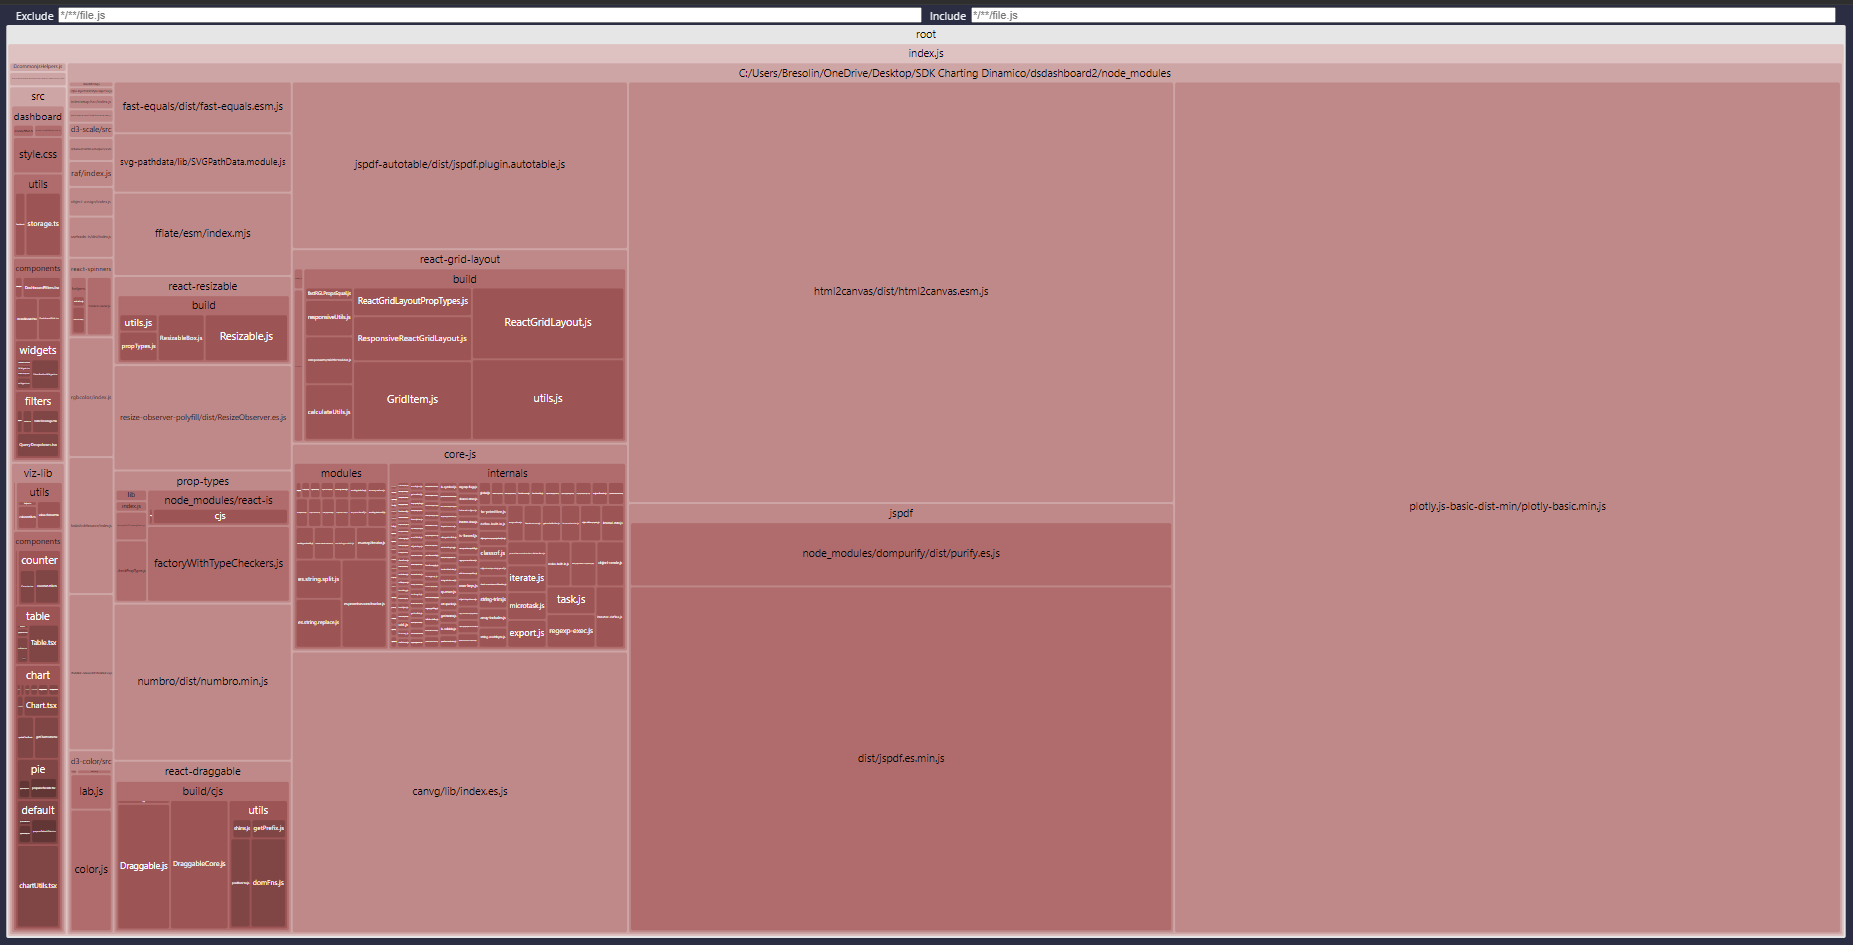
\includegraphics[alt={Esempio di bundle visualizer report}, width=1 \columnwidth]{img/bundle-visualizer.png}
    \caption{Esempio di \textit{bundle visualizer report}}
    \label{fig:bundle-visualizer}
\end{figure}

Per effettuare la build del progetto è necessario eseguire il comando \textit{yarn build-package} configurato all'interno del file \textit{package.json} del progetto:
tale comando, come mostrato nel listato (\S \ref{listing:scripts_package_json_dsdashboard2}), effettua la \textit{build} del progetto generando i file di output all'interno della cartella \textit{dist}.\\
Data la configurazione all'interno del file \textit{rollup.config.js}, il comando effettua la \textit{build} del progetto in formato \textit{ESM} e \textit{CJS}.\\
Per specificare il punto di ingresso per i consumatori dei \textit{package}, sono state definite all'interno del file \textit{package.json} le chiavi \textit{main} e \textit{module} che puntano
rispettivamente ai file \textit{dist/cjs/index.js} e \textit{dist/esm/index.esm.js}.
Per quanto riguarda il rilascio vero e proprio, utilizzando \textit{Yarn} come \textit{package manager}, il rilascio di un \textit{package} può avvenire principalmente tramite tre modalità differenti:
\begin{itemize}
    \item \textbf{Registro di npm}: è il registro di default di \textit{Yarn}, un registro pubblico che permette a chiunque abbia
          un account di pubblicare pacchetti. Per impostazione predefinita (ma comunque configurabile), i pacchetti pubblicati su \textit{npm}
          sono visibili a tutti e di conseguenza tutti possono usufruirne;
    \item \textbf{Registro privato}: è un registro privato che permette di pubblicare pacchetti in un ambiente accessibile solo a chi è
          autorizzato. Esistono differenti servizi che offrono registri privati, a seconda del contesto operativo e delle esigenze dei prodotti
          che devono usufruire di tali pacchetti;
    \item \textbf{Github Packages}: è un \textit{software package hosting service} offerto da \textit{Github} che permette di pubblicare pacchetti
          in modo pubblico o privato all'interno di un repository \textit{Github}, similmente ad un registro \textit{npm}.
\end{itemize}
Per questo progetto si è optato per l'utilizzo di quest'ultima opzione come registro di pubblicazione dei pacchetti, in quanto
all'interno di \textit{Datsoil S.r.l.} i \textit{package} prodotti vengono pubblicati all'interno dello spazio \textit{Github Packages} dell'organizzazione aziendale:
questo servizio è infatti molto utile per chi utilizza \textit{Github} come sistema di versionamento e vuole mantenere i pacchetti all'interno del proprio \textit{repository}.
Per pubblicare un pacchetto all'interno di \textit{Github Packages} è necessario configurare il file \textit{package.json} del progetto, specificando
il campo \textit{publishConfig} nel seguente modo:

\begin{listing}[H]
    \begin{minted}{json}
    {
        "publishConfig": {
            "registry": "https://npm.pkg.github.com/"
        }
    }
    \end{minted}
    \caption{Configurazione del campo \textit{publishConfig} all'interno del file \textit{package.json}}
    \label{listing:package_json_publish_config}
\end{listing}

In seguito, dopo aver configurato il file \textit{.npmrc} all'interno del progetto, specificando il \textit{token} di autenticazione per l'accesso al registro di \textit{Github Packages},
è possibile eseguire il comando \textit{yarn publish} per pubblicare il pacchetto: una volta avviato il comando, verrà illustrata la versione precedente del
\textit{package} e verrà infine richiesto di fornirne una nuova. \\
Una volta terminato il processo di pubblicazione, il pacchetto sarà disponibile all'interno del registro \textit{Github Packages} dell'organizzazione aziendale.

\section{Integrazione SDK all'interno di SYNMGR}
Durante lo svolgimento dello stage ho avuto la possibilità di integrare l'SDK prodotto all'interno del prodotto \textit{SYNMGR} di \textit{Datasoil S.r.l.},
l'applicazione web di test utilizzata dall'azienda per testare gli sviluppi futuri e le nuove funzionalità che verranno in seguito rilasciate sul prodotto ufficiale \textit{SYN}. \\
Per utilizzare l'SDK all'interno di \textit{SYNMGR} è stato necessario configurare il file \textit{.npmrc} all'interno del progetto, specificando il \textit{token} di autenticazione
per l'accesso al registro di \textit{Github Packages}: utilizzando infatti il registro fornito da \textit{Github}, i package manager come \textit{Yarn} e \textit{npm} andranno
a verificare la presenza di tali informazioni e, solo nel caso di riscontro positivo, permetteranno l'installazione dei pacchetti richiesti. \\
Successivamente è stata sostituito il precedente SDK \textit{dsdashboard} a favore del nuovo SDK \textit{dsdashboard2} all'interno del file \textit{package.json} del progetto,
eseguendo infine il comando \textit{yarn install} per l'installazione del pacchetto, permettendo di utilizzare all'interno del prodotto le nuove implementazioni
delle componenti inerenti alle dashboard.

\begin{listing}[H]
    \begin{minted}{json}
    {
        "dependencies": {
            "@datasoil/dsdashboard2": "^0.1.5"
        }
    }
    \end{minted}
    \caption{Configurazione del campo \textit{dependencies} all'interno del file \textit{package.json} di \textit{SYNMGR}}
    \label{listing:package_json_synmgr}
\end{listing}

Di seguito, un esempio di una dashboard presente all'interno di \textit{SYNMGR} che utilizza l'SDK \textit{dsdashboard2}.

\begin{figure}[H]
    \centering
    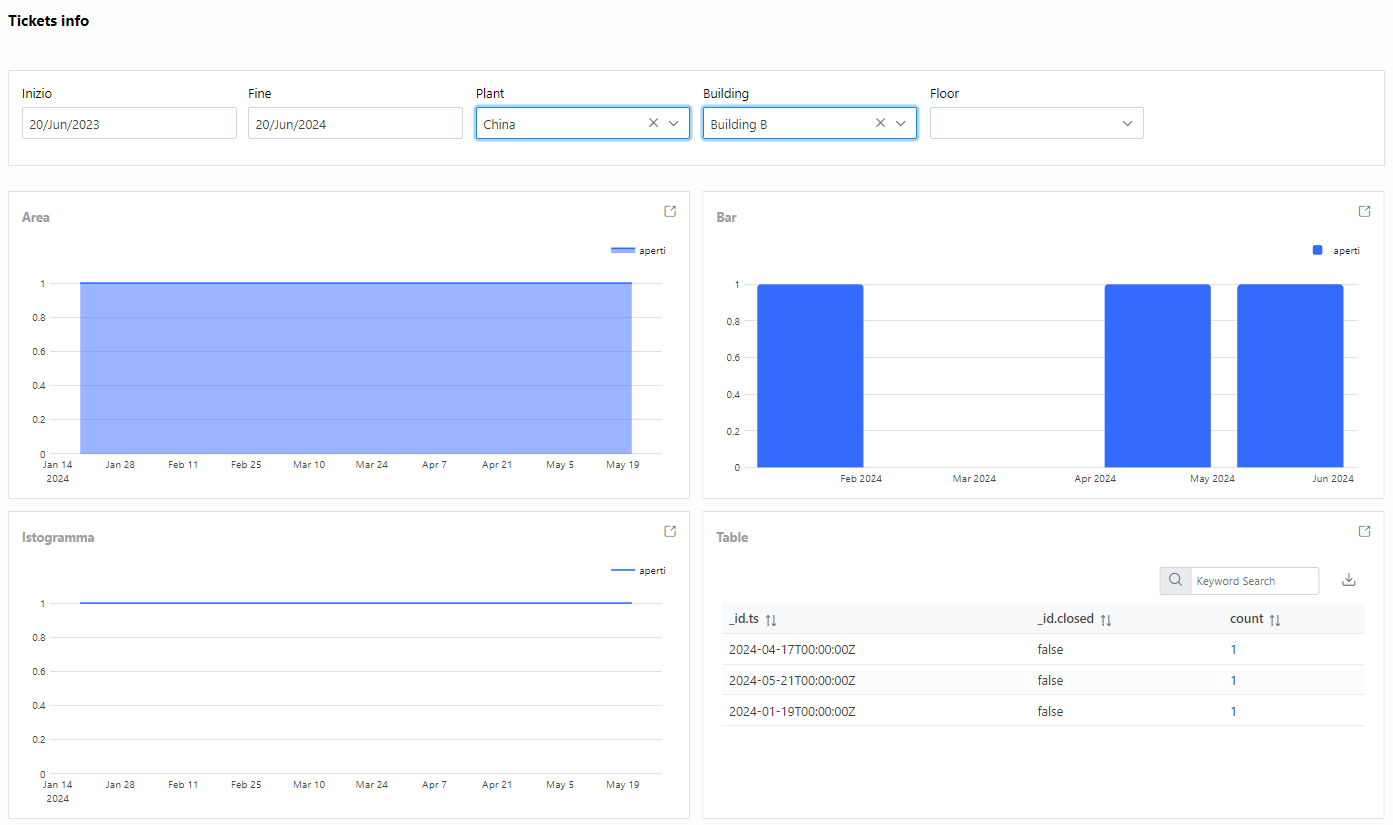
\includegraphics[alt={Esempio di dashboard all'interno di SYNMGR}, width=1 \columnwidth]{img/synmgr-dashboard.png}
    \caption{Esempio di dashboard all'interno di \textit{SYNMGR}}
    \label{fig:synmgr_dashboard}
\end{figure}